\section{Техническое задание}
\subsection{Основание для разработки}

Основанием для разработки является задание на производственную преддипломную практическую работу в компании "<ООО МЦОБ. Онлайн Сервисы">.

\subsection{Цель и назначение разработки}

Основной задачей производственной преддипломной практической работы является разработка программной системы для визуализации трёхмерных данных, использующая библиотеку OpenGL.

Используя библиотеку OpenGL последней версии, планируется разработать приложение на языке C\#, способное импортировать массив трёхмерных данных и визуализировать их в виде трёхмерных моделей.

Задачами данной разработки являются:
\begin{itemize}
\item создание программы, реализующей графику, на основе спецификации OpenGL;
\item реализация программы парсера, способного преобразовывать и загружать в программу трёхмерные данные;
\item разработка интерфейса для взаимодействия с программой;
\item реализация функции хранения и загрузки трёхмерных данных внутри программы.
\end{itemize}

\subsection{Требования к программной системе}

\subsubsection{Требования к данным программно-информационной системы}

Входными данными для программной системы являются файлы с расширением *.obj, внутри которых содержатся информация в виде массивов трёхмерных данных; файлы текстур - изображения с расширением *.png и *.jpg; данные ввода с клавиатуры и мыши, которые служат для управления перемещением и вращением камеры.

Выходными данными для программной системы является выводимое на экран изображение двумерной проекции трёхмерных объектов на виртуальной сцене.

На рисунке ~\ref{diagram1:image} представлена диаграмма описания потоков данных в программе.

\begin{figure}[ht]
	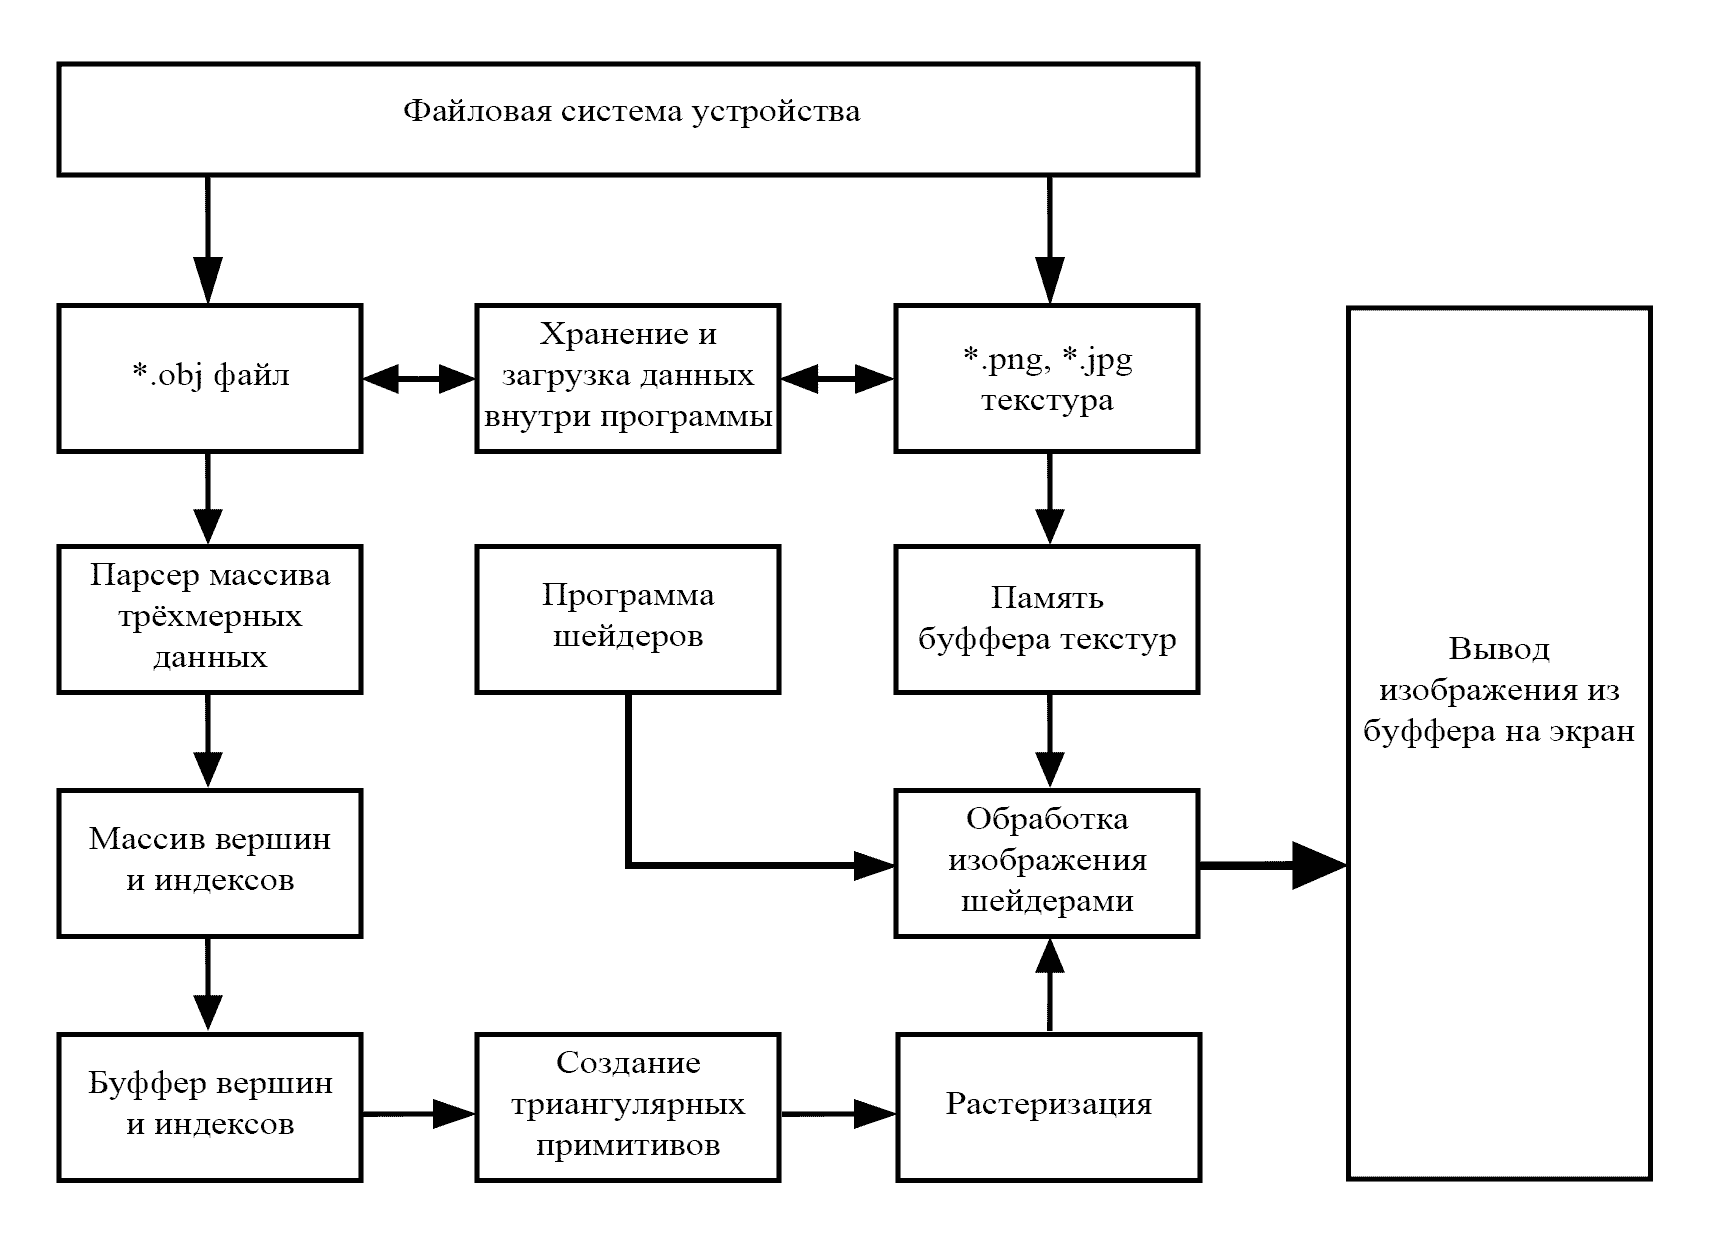
\includegraphics[width=1\linewidth]{diagram1}
	\caption{Диаграмма потоков данных в программе}
	\label{diagram1:image}
\end{figure}

\subsubsection{Функциональные требования к программной системе}

Программа должна реализовывать следующие функции:
\begin{itemize}
    \item позволять пользователю импортировать любые массивы трёхмерных данных (включая текстуры для трёхмерных моделей);
    \item выполнять отрисовку трёхмерной сцены в реальном времени (каждый кадр);
    \item пользволять пользователю свободно управлять перспективой виртуальной камеры;
    \item предоставлять возможность преобразовывать массив трёхмерных данных (производить аффинные преобразования) в рамках: сдвига, вращения и растяжения (сжатия);
    \item импортировать, хранить и загружать массив трёхмерных данных внутри самой программы.
\end{itemize}



Виды преобразований массива трёхмерных данных, предоставляемых программой, представлены на рисунке ~\ref{affin:image}.

\begin{figure}[ht]
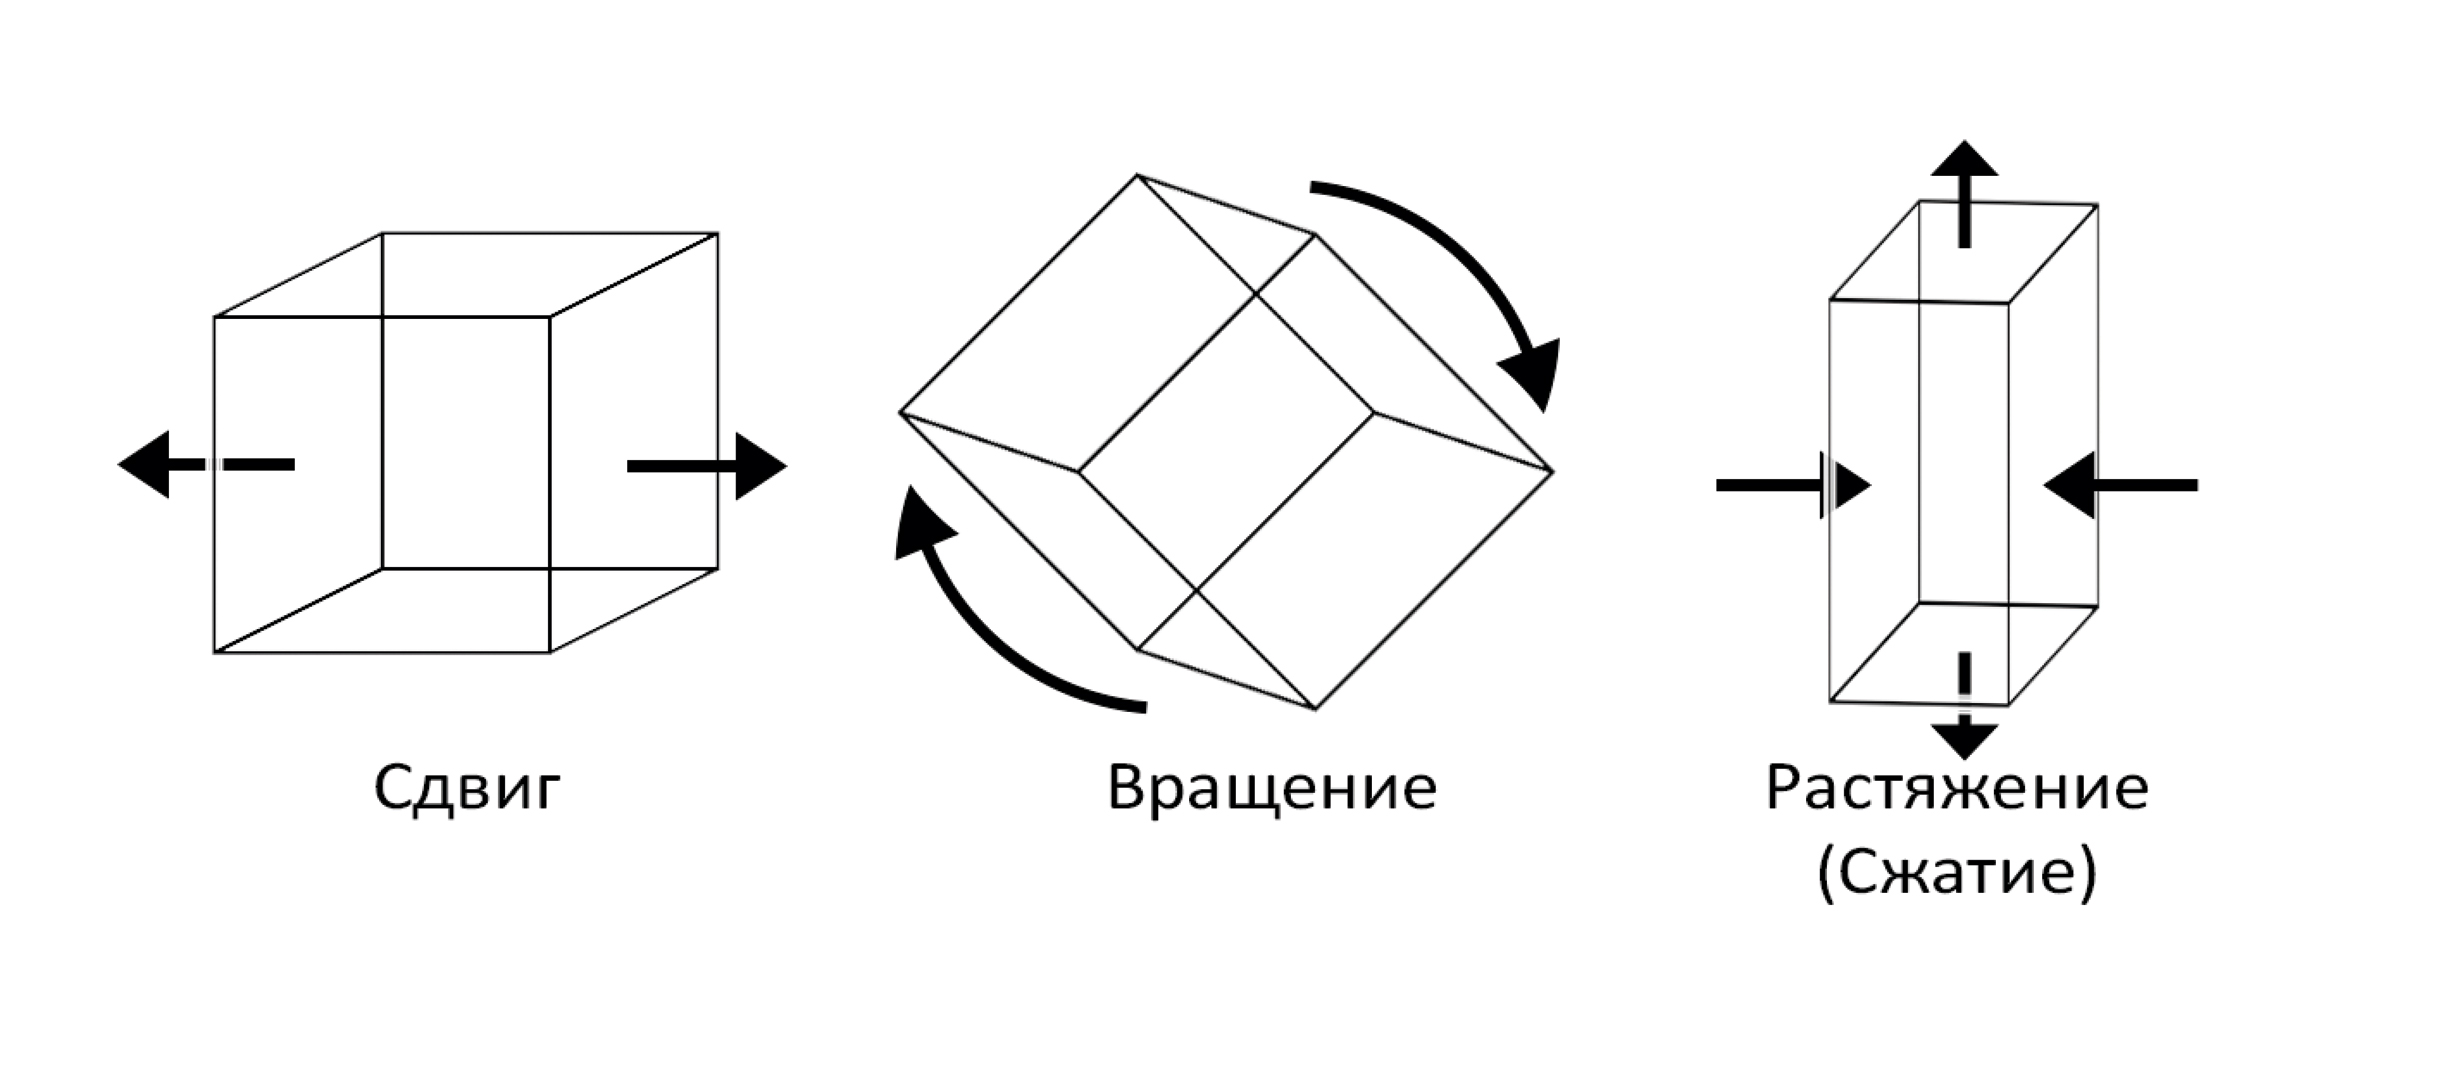
\includegraphics[width=1\linewidth]{affin}
\caption{Виды преобразований массива трёхмерных данных}
\label{affin:image}
\end{figure}
%\vspace{-\figureaboveskip} % двойной отступ не нужен (можно использовать, если раздел заканчивается картинкой)

\subsubsection{Требования к графическому интерфейсу программы}

Программное обеспечение должно иметь минимальный, но содержательный и интуитивный интерфейс. Большую часть основного окна приложения должно занимать само окно вывода растрового изображения проекции виртуальной сцены и всех трёхмерных данных на ней. Сбоку на основном окне приложения должно находиться специально выведенное отдельное окно «инспектора», с помощью которого пользователь сможет управлять загрузкой и сохранением массивов трёхмерных данных, а также взаимодействовать с уже существующими данными на виртуальной сцене.

Макет пользовательского интерфейса, составленный по данным требованиям представлен на рисунке ~\ref{maket1:image}

\begin{figure}[ht]
	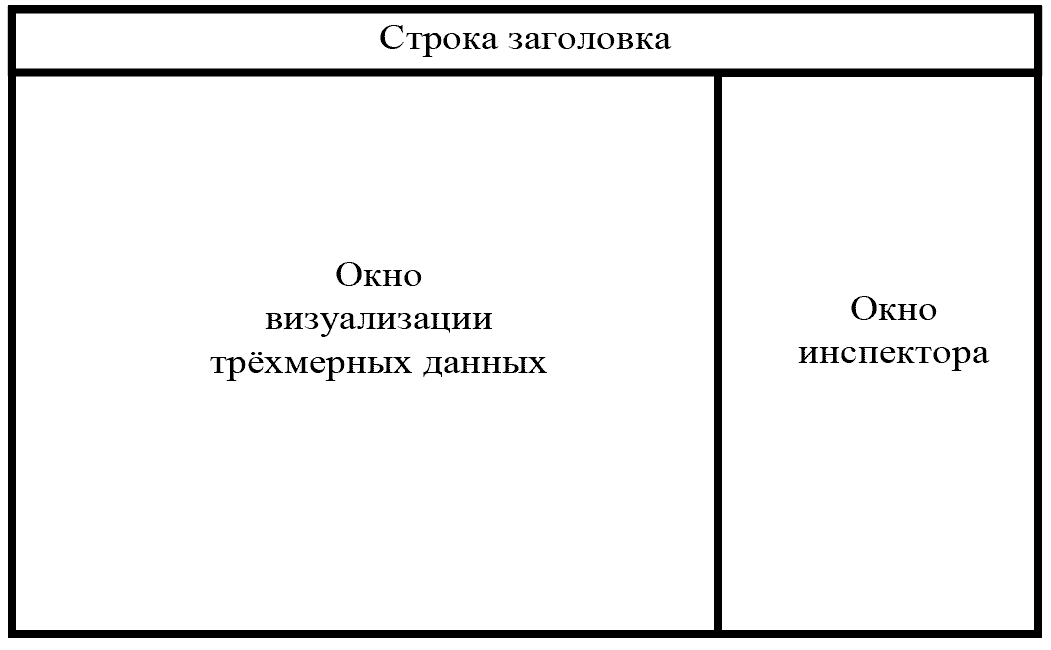
\includegraphics[width=1\linewidth]{maket1}
	\caption{Макет пользовательского интерфейса}
	\label{maket1:image}
\end{figure}

\subsection{Моделирование вариантов использования}

Для разрабатываемого программного обеспечения была реализована модель, которая демонстрирует наглядное представление вариантов использования программы.

На основании анализа предметной области в программе должны быть реализованы следующие прецеденты:
\begin{enumerate}
\item Импортирование массивов трёхмерных данных из файловой системы пользователя.
\item Просмотр визуализированного массива трёхмерных данных в виде отрисованных объектов на экране.
\item Осуществление трансформаций над массивом трёхмерных данных.
\item Хранение и загрузка массивов трёхмерных данных.
\end{enumerate}

На рисунке ~\ref{diagram2:image} представлена диаграмма вариантов использования

\begin{figure}[H]
	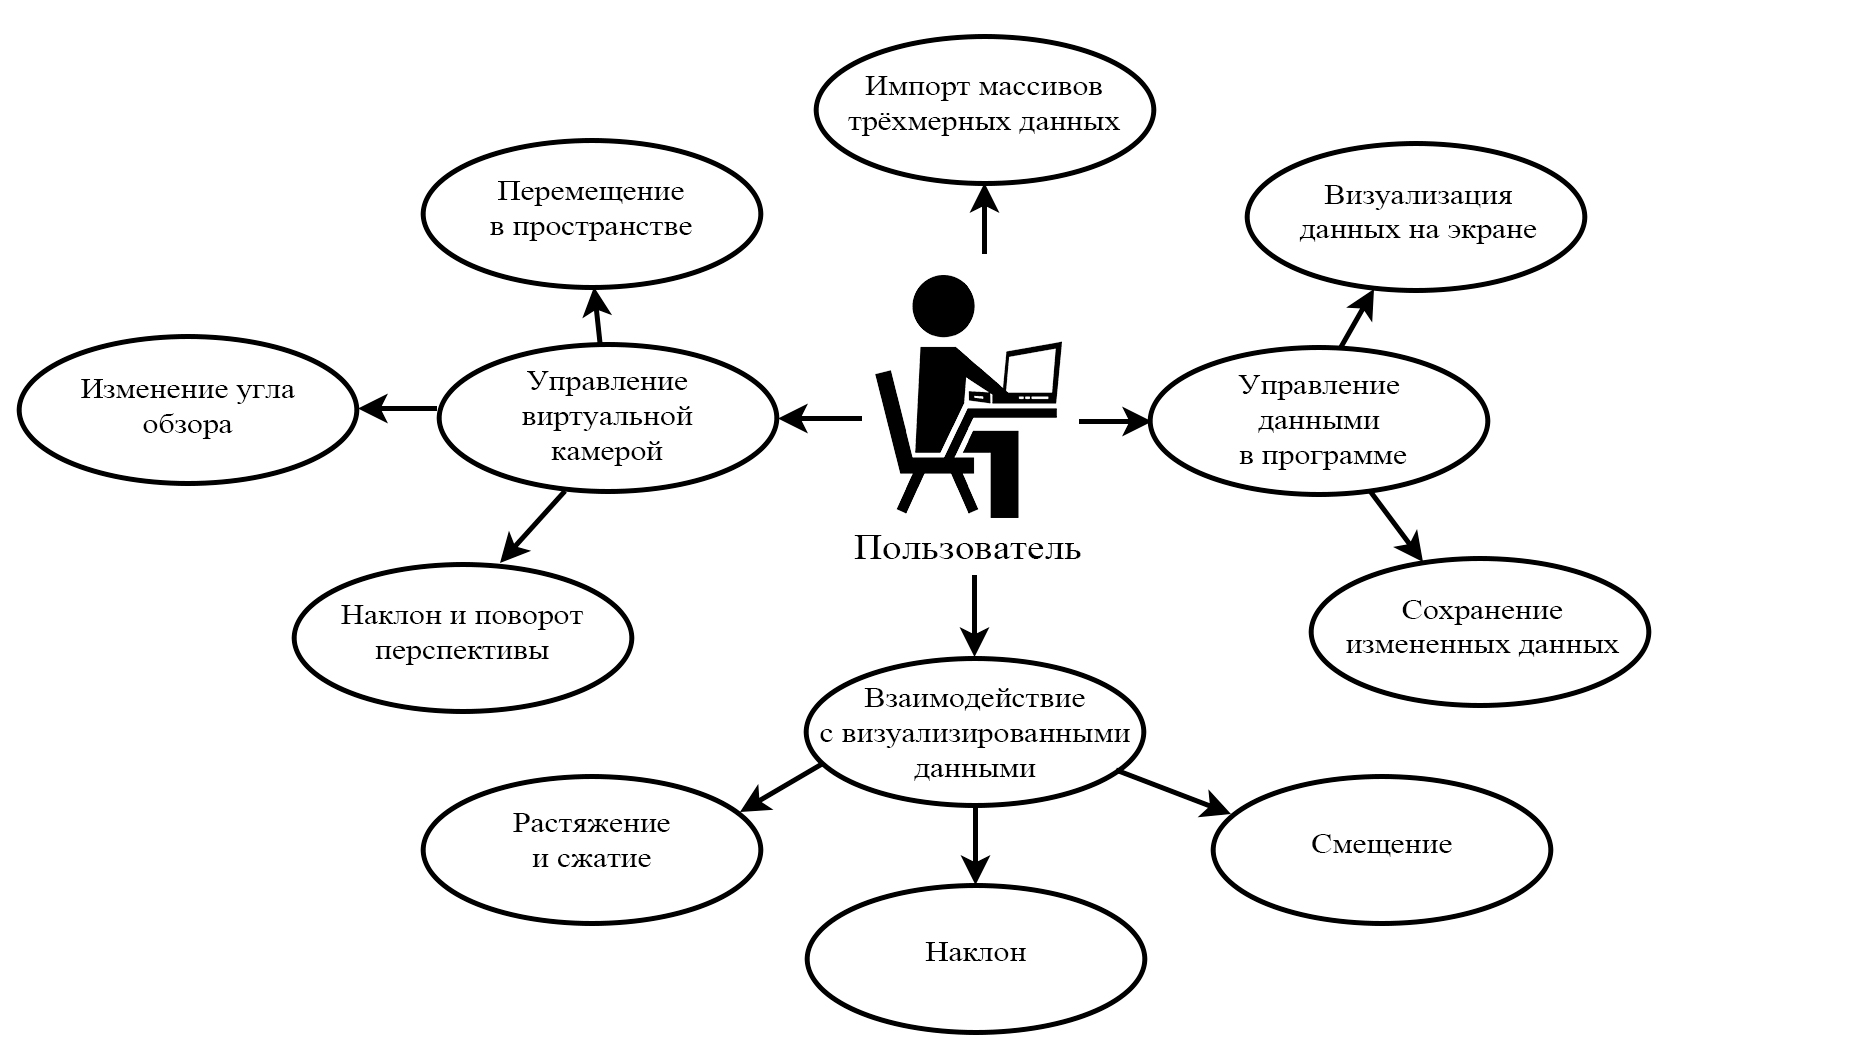
\includegraphics[width=1.1\linewidth]{diagram2}
	\caption{Диаграмма вариантов использования}
	\label{diagram2:image}
\end{figure}

\subsection{Нефункциональные требования к программной системе}

Требования к аппаратной совместимости:
\begin{itemize}
	\item видеоадаптер с поддержкой OpenGL версии не ниже 4.6;
	\item минимальное разрешение экрана - 800х600 пикселей.
\end{itemize}

Требования к программной совместимости:
\begin{itemize}
	\item операционная система x86 Windows 7 и выше;
	\item система, с установленными компонентами Microsoft Visual C++ версии 2015 года и выше.
\end{itemize}

\subsection{Требования к оформлению документации}

Разработка программной документации и программного изделия должна производиться согласно ГОСТ 19.102-77 и ГОСТ 34.601-90. Единая система программной документации.

